\documentclass[twocolumn]{article}
\usepackage{graphicx}
\usepackage{amsmath}
\usepackage{float}
\usepackage{amssymb} %Use of therefore symbol
\usepackage{hyperref}
\usepackage{caption}



\begin{document}
\title{Lab 1: Monte Carlo Methods}
\author{Alex Matheson, Austin Nhung}
%\affiliation{Department of Physics and Astronomy, University of Calgary, Calgary AB T2N 1N4 Canada}
\date{\today}
\maketitle

\section{Introduction}

\section{Methods}
Fourier series are defined by calculating the fourier coefficients $a_n$ and $b_n$. These coefficients may be replaced when in a complex fourier series using a term $c_n$. Using the following equations:
\begin{equation}
\begin{split}
a_n =& c_n + c_{-n} \\
b_n =& i(c_n - c_{-n}) \\
c_n =& \frac{1}{2}(a_n - ib_n)
\end{split}
\end{equation}
In fourier series, the $a_n$ and $b_n$ correspond to even and odd 'components' of the function. In the case of an even function:
\begin{equation}
\begin{split}
a_n =& c_n + c_{-n} \\
b_n =& 0 \\
c_n =& \frac{1}{2}(a_n)
\end{split}
\end{equation}

And for odd functions:
\begin{equation}
\begin{split}
a_n =& 0 \\
b_n =& i(c_n - c_{-n}) \\
c_n =& \frac{-ib_n}{2}
\end{split}
\end{equation} 
 
It may be shown in both of the above series that the $a_n$ term for even functions and $b_n$ for odd functions will be proportional to the $c_n$ terms. 

Next, a square wave function was considered as defined below: 

\[ 
f(t)=
\begin{cases}
1, & |t| \leq T/4 \label{eq:square}
\\
0, & |t| > T/4
\end{cases}
\]

This function was periodic between $-T/2$ and $T/2$. The function was visualized in figure \ref{fig:square}. As with any function, this could be re-stated using complex Fourier series. To compute the series, the coefficients $c_n$ were determined according to equation \ref{eq:complex_coefficients}. 

\begin{figure}
\centering
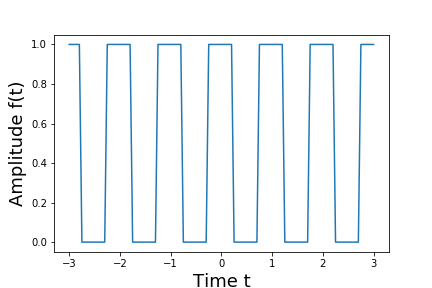
\includegraphics[width=\linewidth]{Figure1}
\caption{A square wave function. The period of the function has been set to $T=1$, periodic from $T=-1/2$ to $T=1/2$.}
\label{fig:square}
\end{figure}

\begin{equation}
c_n = \frac{1}{T} \int_{-T/2}^{T/2} f(t) \exp(-i\frac{2\pi nt}{T}) dt
\label{eq:complex_coefficients}
\end{equation}

The coefficients could be solved analytically, yielding the answer $c_n = \frac{-i}{\pi n}$ for $n = 1, 3, 5, ...$. As the found $n$ values suggest, the original function was purely odd, meaning that the function could be constructed from purely sine terms. Due to this, all even $c_n$ terms (including $c_0$) are $0$. The values of the different $c_n$ terms may also be plotted, as shown in figure \ref{fig:Figure2}. The values in this plot show that the odd $n$ terms follow a hyperbolic sinusoid path. The complete series may be written as:

\[
f(t) = \sum_{n= -\infty}^{\infty} -\frac{i}{\pi n} \exp(-i \frac{2\pi nt}{T})
\]

\begin{figure}
\centering
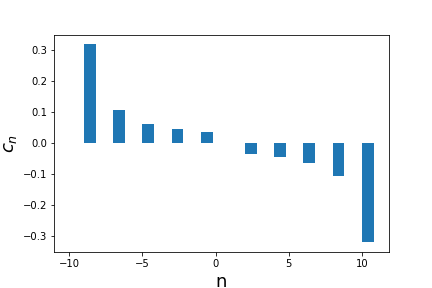
\includegraphics[width=\linewidth]{Figure2}
\caption{Values of each term $c_n$ in the complex fourier series.}
\label{fig:Figure2}
\end{figure}

\subsection{Noise}
\subsubsection{Autocorrelation and PSD}
The autocorrelation function was examined in a previous lab. It turns out that the auto-correlation function may be applied to random signals (i.e. noise) as well. For white noise created from a uniform distribution of frequencies, the autocorrelation function is expected to be a delta function. Consider an ideal random number generator separate from the realities of computing. By definition, a number correlates with itself completely, forming a spike at $k=0$. For ideal noise, there is no relation between the first number generated, and any subsequent number generated. This means that subsequent values should yield $k=0$. Taken together, this is a description of $\delta(k)$.

The power spectral density function is connected to the auto-correlation function by the following formula:

\[ S(\omega) = \sum_{-\infty}^{\infty} AC(k)e^{-j\omega k} \]

Using this, the PSD of white noise may be calculated:

\[ S(\omega) =  \sum_{i=-\infty}^{\infty} \delta (k) e^{-j\omega k}\\
S(\omega) = \delta(k=0) e^{-j\omega * 0} \\
S(\omega) = 1
  \] 


\subsection{Applications}
\subsubsection{ODEs and the Fourier Transform}
The Fourier transform can be use to reduce the dimensionality of a differential equation. In essence, if the fourier transform is used, a PDE with two different differentials may be reduced to an ODE or and ODE to a polynomial equation. The original solution may then be recovered by reverse transforming the result. Below are a few examples of simplifying differential equations through Fourier transform:

\begin{equation}
\begin{split}
\mathcal{F} \{ m\ddot{x} + D\dot{x} + \kappa x &= n(t) \} \\
-\omega^2 \hat{x} +i\omega \hat{x} + \kappa\hat{x} &= \hat{n}(\omega)
\end{split}
\end{equation}

\begin{equation}
\begin{split}
\mathcal{F} \{ih \frac{\partial \psi}{\partial t} + \frac{h^2}{2m} \frac{\partial^2 \psi}{\partial x^2} &= 0 \} \\
-\omega h \hat{\psi} - \frac{ih^2}{2m} \frac{\partial^2 \hat{\psi}}{\partial x^2} = 0
\end{split}
\end{equation}

\begin{equation}
\begin{split}
\mathcal{F} \{ \frac{\partial^2 T}{\partial x^2} + \frac{\partial^2 T}{\partial z^2} &= \delta (x) \delta (z - a) \}\\
-k^2 \hat{T} + \frac{\partial^2 \hat{T}}{\partial z^2} &= e^{-2\pi ik x} \delta (z - a)
\end{split}
\end{equation}

\subsubsection{Heat Equation}
A common differential equation that is difficult to solve with non-complex analysis was the heat equation. The heat equation was defined as:
\begin{equation}
\begin{split}
\frac{\partial^2 T}{\partial x^2} &= -q(x)\\
q(x) =& \frac{\exp(-(x-x_0)^2/(2\sigma^2))}{\sqrt{2\pi\sigma^2}}
\end{split}
\end{equation}

This equation may be re-written using Fourier analysis. Two aids were used in this analysis: an integral table result for a zero-mean gaussian transform \cite{gauss_trans}, and the Fourier shift theorem to take care of the $x_0$ shift. Equations \ref{eq:gauss_transform} show this process.

\begin{equation}
\begin{split}
&\mathcal{F}\{ \frac{\partial^2 T}{\partial x^2} \} = \mathcal{F} \{ -q(x) \} \\
&-k^2 \hat{T} = -\hat{q}(x) \\
&\\
\hat{q}(x) =& \mathcal{F} \{ \frac{\exp(-(x-x_0)^2/(2\sigma^2))}{\sqrt{2\pi\sigma^2}} \} \\
\hat{q}(x) =& e^{-2\pi ikx_0} \times \mathcal{F} \{ \frac{\exp(-(x^2/(2\sigma^2))}{\sqrt{2\pi\sigma^2}} \} \\
\hat{q}(x) =& \exp\bigg( \frac{-\sigma^2 k^2}{2} - 2\pi ikx_0 \bigg) \\
\hat{T} =& \frac{1}{k^2} \exp\bigg( \frac{-\sigma^2 k^2}{2} - 2\pi ikx_0 \bigg)
%
%\hat{q}(x) =& \frac{1}{\sqrt{2\pi\sigma^2}} \int_{-\infty}^{\infty} e^{2\pi ikx} e^{-(x-x_0)^2/\sqrt{2\sigma^2}} dx \\
%\hat{q}(x) =& \frac{1}{\sqrt{2\pi\sigma^2}} \int_{-\infty}^{\infty} \cos(2\pi kx) e^{-(x-x_0)^2/\sqrt{2\sigma^2}} dx \\
%\hat{q}(x) =& \frac{1}{\sqrt{2\pi\sigma^2}} e^{-2\pi ikx_0} \int_{-\infty}^{\infty} \cos(2\pi kx) e^{-x^2/\sqrt{2\sigma^2}} dx \\
%\hat{q}(x) =& \frac{1}{\sqrt{2\sigma^2}} e^{-2\pi ikx_0} \sqrt{\pi\sqrt{2\pi\sigma^2}} e^{-\pi^2 k^2 \sqrt{2\sigma^2}} \\
%\hat{T} &= \frac{e^{-\pi^2 k^2\sqrt{2\sigma^2} - 2\pi ikx_0/(2\sigma)^2}}{\sqrt{2k\pi\sigma^2}}
\end{split}
\label{eq:gauss_transform}
\end{equation}

In order to obtain a solution to the heat equation, a reverse transform could be applied on the above equation to return the original heat function.

\section{Conclusion}



\begin{thebibliography}{00}
	\bibitem{ouyed}
	Ouyed and Dobler, PHYS 581 course notes, Department of Physics and Astrophysics, University of Calgary (2016).
	\bibitem{NR}
	W. Press et al., \emph{Numerical Recipes} (Cambridge University Press, 2010) 2nd. Ed.
	\bibitem{Code}
	C. Hass and J. Burniston, MCMC Hill Climbing. Jupyter notebook, 2018.
	\bibitem{gauss_trans}
	K. Derpanis, Fourier Transform of the Gaussian, 2005, accessed at \url{http://www.cse.yorku.ca/~kosta/CompVis_Notes/fourier_transform_Gaussian.pdf}.
\end{thebibliography}

\section{Appendix}
For access to the source codes used in this project, please visit \url{https://github.com/Tsintsuntsini/PHYS_581} for a list of files and times of most recent update.
	
\end{document}